
\documentclass[11pt,oneside]{report}

\usepackage[T1]{fontenc}
\usepackage[utf8]{inputenc}
\usepackage{lmodern}
\usepackage[a4paper,margin=1in]{geometry}
\usepackage{microtype}
\usepackage{setspace}
\usepackage{amsmath,amssymb}
\usepackage{booktabs,longtable,tabularx,array}
\usepackage{graphicx}
\usepackage{enumitem}
\usepackage{hyperref}
\usepackage{fancyhdr}
\usepackage{titlesec}
\usepackage{tikz}
\usetikzlibrary{arrows.meta,positioning,shapes.geometric,fit,calc}
\usepackage[most]{tcolorbox}
\usepackage{listings}
\usepackage{xcolor}
\usepackage{ragged2e}
\usepackage{multicol}
\usepackage{etoolbox}

\raggedbottom
\setstretch{1.12}
\setlength{\parindent}{0pt}
\setlength{\parskip}{0.55em}
\setlength{\emergencystretch}{3em}
\setlist[itemize]{leftmargin=1.5em,itemsep=0.35em,topsep=0.35em}
\setlist[enumerate]{leftmargin=1.7em,itemsep=0.35em,topsep=0.35em}
\renewcommand{\arraystretch}{1.2}
\setcounter{tocdepth}{1}

\definecolor{TitleBlue}{HTML}{173B6C}
\definecolor{AccentTeal}{HTML}{0F766E}
\definecolor{AccentGold}{HTML}{A16207}
\definecolor{SoftBlue}{HTML}{EEF4FB}
\definecolor{SoftTeal}{HTML}{EDF9F7}
\definecolor{SoftGold}{HTML}{FBF7E8}
\definecolor{SoftRed}{HTML}{FDF1F1}
\definecolor{SoftPurple}{HTML}{F4F0FB}
\definecolor{LineGray}{HTML}{D8DEE8}
\definecolor{BodyGray}{HTML}{333333}
\definecolor{DeepRed}{HTML}{9F2D2D}
\definecolor{DeepPurple}{HTML}{5F3A9B}
\definecolor{SoftGray}{HTML}{F8FAFC}

\newcommand{\GuideTitle}{Retrieval from Zero}
\newcommand{\GuideAuthor}{Soroosh Aghaei}

\color{BodyGray}
\hypersetup{
  colorlinks=true,
  linkcolor=TitleBlue,
  urlcolor=AccentTeal,
  pdftitle={\GuideTitle},
  pdfauthor={\GuideAuthor},
  pdfsubject={Information retrieval study guide from beginner foundations to full pipeline understanding}
}

\pagestyle{fancy}
\fancyhf{}
\fancyhead[L]{\footnotesize\color{TitleBlue}\textsf{Retrieval from Zero}}
\fancyhead[R]{\footnotesize\color{AccentTeal}\textsf{\nouppercase{\leftmark}}}
\fancyfoot[C]{\footnotesize\thepage}
\setlength{\headheight}{15pt}
\renewcommand{\headrulewidth}{0.4pt}
\renewcommand{\footrulewidth}{0pt}

\titleformat{\part}[display]
  {\normalfont\bfseries\Huge\color{TitleBlue}}
  {\filright\Huge Part \thepart}
  {0.8ex}
  {\titlerule[1pt]\vspace{1ex}\filright\LARGE}
  [\vspace{1ex}\titlerule]

\titleformat{\chapter}[display]
  {\normalfont\bfseries\color{TitleBlue}}
  {\filleft\Huge\thechapter}
  {0.5ex}
  {\titlerule[1pt]\vspace{0.8ex}\filright\LARGE}
  [\vspace{0.8ex}\titlerule]

\newtcolorbox{purposebox}{
  colback=SoftBlue,colframe=TitleBlue,
  title=Why this chapter exists,
  fonttitle=\bfseries,
  breakable
}

\newtcolorbox{intuitionbox}[1][]{
  colback=SoftTeal,colframe=AccentTeal,
  title={Practical intuition#1},
  fonttitle=\bfseries,
  breakable
}

\newtcolorbox{examplebox}[1][]{
  colback=white,colframe=AccentTeal,
  title={Tiny worked example#1},
  fonttitle=\bfseries,
  breakable
}

\newtcolorbox{warningbox}[1][]{
  colback=SoftRed,colframe=DeepRed,
  title={Common mistake#1},
  fonttitle=\bfseries,
  breakable
}

\newtcolorbox{rememberbox}[1][]{
  colback=SoftGold,colframe=AccentGold,
  title={If you feel lost, remember this#1},
  fonttitle=\bfseries,
  breakable
}

\newtcolorbox{selfcheckbox}[1][]{
  colback=SoftPurple,colframe=DeepPurple,
  title={Self-check#1},
  fonttitle=\bfseries,
  breakable
}

\newtcolorbox{answerbox}[1][]{
  colback=SoftGray,colframe=LineGray,
  title={Short answers#1},
  fonttitle=\bfseries,
  breakable
}

\newtcolorbox{notebox}[1][]{
  colback=SoftGray,colframe=LineGray,
  title={Do not memorize this yet#1},
  fonttitle=\bfseries,
  breakable
}

\newtcolorbox{formulabox}[1][]{
  colback=white,colframe=TitleBlue,
  title={Formal version#1},
  fonttitle=\bfseries,
  breakable
}

\newcommand{\term}[1]{\textbf{#1}}
\newcommand{\vect}[1]{\mathbf{#1}}
\newcommand{\code}[1]{\texttt{#1}}
\newcolumntype{Y}{>{\RaggedRight\arraybackslash}X}
\newcolumntype{C}{>{\Centering\arraybackslash}X}

\lstdefinestyle{plaincode}{
  basicstyle=\ttfamily\small,
  breaklines=true,
  frame=single,
  framerule=0.5pt,
  rulecolor=\color{LineGray},
  backgroundcolor=\color{SoftGray},
  columns=fullflexible,
  keepspaces=true
}
\lstset{style=plaincode}

\newcommand{\chapterpattern}{%
\begin{rememberbox}
Each chapter tries to follow the same learning rhythm: why the idea exists, what problem it solves, a toy example, a more technical explanation, a careful formal version, a warning about common confusion, and a few small questions so you can check whether the idea really made sense.
\end{rememberbox}}

\makeatletter
\newcommand{\compacttableofcontents}{%
  \chapter*{\contentsname}
  \@mkboth{\MakeUppercase\contentsname}{\MakeUppercase\contentsname}%
  \begingroup
  \setlength{\parskip}{0pt}%
  \setlength{\columnsep}{1em}%
  \footnotesize
  \setstretch{0.9}%
  \begin{multicols}{2}
  \@starttoc{toc}%
  \end{multicols}
  \endgroup
}
\makeatother

\begin{document}

\begin{titlepage}
\thispagestyle{empty}

\begin{tikzpicture}[remember picture,overlay]
\fill[TitleBlue] (current page.north west) rectangle (current page.south east);
\fill[white,opacity=0.08] ([xshift=-1cm,yshift=-2cm]current page.north east) circle (4cm);
\fill[white,opacity=0.08] ([xshift=1cm,yshift=3cm]current page.south west) circle (5cm);
\node[anchor=north west,text width=0.78\paperwidth,align=left,text badly ragged] at ([xshift=1in,yshift=-1.25in]current page.north west) {\color{white}\bfseries\fontsize{28}{32}\selectfont \GuideTitle\\[0.4em]A beginner's guide to retrieval, reranking, evaluation,\\and end-to-end search pipelines};
\node[anchor=north west,text width=0.68\paperwidth,align=left] at ([xshift=1in,yshift=-4.45in]current page.north west) {\color{white}\Large Start with the foundations of text, vectors, similarity, and ranking. Then build toward TF--IDF, BM25, embeddings, bi-encoders, cross-encoders, category-aware reranking, and reliable evaluation.};
\node[anchor=south west,text width=0.75\paperwidth,align=left] at ([xshift=1in,yshift=1.1in]current page.south west) {\color{white}\large A self-contained study path with worked examples, diagrams, glossaries, and self-checks.\\[0.8em]\textbf{Author:} \GuideAuthor};
\end{tikzpicture}
\vfill
\end{titlepage}

\pagenumbering{roman}
\chapter*{How to Use This Guide}
\addcontentsline{toc}{chapter}{How to Use This Guide}
This document is designed for a student who has no stable base yet. It is not a compressed revision sheet. It is a teaching document. Read it in order on the first pass. On the second pass, pause often and solve the self-checks before reading the answers. On the third pass, connect the ideas to the actual notebook and its implementation choices.

There are three important promises behind the structure.
\begin{itemize}
\item \term{Nothing important is assumed.} Words such as feature, vector, relevance, candidate set, reranker, or leakage are taught before they are used heavily.
\item \term{Formulas come late.} The guide first answers the question ``what problem does this solve?'' and only then gives symbols.
\item \term{The notebook comes after the concepts.} The goal is to understand the system, not to memorize variable names blindly.
\end{itemize}

\chapterpattern

\compacttableofcontents

\clearpage
\pagenumbering{arabic}
\part[Foundations]{Before Retrieval: the beginner foundations}
\chapter[Data Science in Plain Language]{What data science is, in plain language}

\begin{purposebox}
Before learning retrieval, you need a small mental toolkit for thinking about data-driven systems. Without that toolkit, later words such as feature, label, model, training, and evaluation feel abstract and disconnected.
\end{purposebox}

\section*{Intuition in ordinary language}
Data science is the practice of learning something useful from organized observations. The observations may come from customers, machines, experiments, documents, clicks, medical records, or forum posts. A data scientist tries to answer questions such as: what pattern is present, what can be predicted, what items look similar, or which option should be ranked first.

A good first picture is this: you collect many examples, you choose what information from each example to look at, you decide what outcome matters, and you build a system that uses the past examples to behave better on new ones.

\begin{intuitionbox}
If a teacher has many old exam papers and their grades, the papers are \term{data}. The characteristics she notices, such as number of solved questions or number of conceptual mistakes, are \term{features}. The final grade is the \term{label}. A system that learns how these characteristics connect to the grade is a \term{model}.
\end{intuitionbox}

\section*{Concrete toy example}
Imagine a tiny email problem. You want to decide whether an email is spam.
\begin{itemize}
\item Email A contains ``win money now'' and many links.
\item Email B contains ``meeting moved to 3pm'' and no suspicious phrases.
\end{itemize}
You might choose these features: number of links, whether the phrase ``win money'' appears, whether the sender is known, and email length. The label is one word: \term{spam} or \term{not spam}.

A rule-based system might say: ``if the email contains the phrase `win money', call it spam.'' A learned system instead looks at many examples and discovers which combinations of features usually lead to spam.

\section*{Technical explanation}
Here are the beginner definitions that matter most.
\begin{itemize}
\item \term{Data}: recorded examples.
\item \term{Feature}: a measurable description of one example.
\item \term{Label}: the outcome or target we want to predict, if one exists.
\item \term{Model}: a mathematical rule that turns input information into an output.
\item \term{Training}: adjusting the model using past labeled examples.
\item \term{Prediction}: using the trained model on a new example.
\item \term{Evaluation}: checking whether the model performs well enough on data that were not used to fit it.
\end{itemize}

Not all data science is prediction. Some tasks are about grouping similar items, detecting anomalies, ranking search results, or summarizing patterns. Retrieval will later fall into the ranking family.

\begin{formulabox}
A labeled dataset is often written as pairs $(x_i,y_i)$.
\begin{itemize}
\item $x_i$ means the input for example $i$.
\item $y_i$ means the desired output for example $i$.
\end{itemize}
For spam filtering, $x_i$ could be one email represented by features, and $y_i$ could be the label \emph{spam} or \emph{not spam}.
\end{formulabox}

\section*{Rule-based systems versus learned systems}
A \term{rule-based system} uses instructions written directly by a human. A \term{learned system} uses data to estimate the instructions. Rule-based systems are often transparent and fast to build when the pattern is simple. Learned systems are often stronger when the pattern is messy, subtle, or too large to encode by hand.

\begin{warningbox}
A learned system is not magical. It still depends on human choices: what data were collected, which features were built, what metric was optimized, and what counts as good performance.
\end{warningbox}

\begin{notebox}
Do not memorize the phrase ``model'' as something mysterious. For now, a model is just a function that takes input and produces an output. The sophistication comes later.
\end{notebox}

\begin{selfcheckbox}
\textbf{1.} In the spam example, name one possible feature and one possible label.\\
\textbf{2.} What is the difference between training and prediction?\\
\textbf{3.} Give one situation where a rule-based system might be enough.
\end{selfcheckbox}

\begin{answerbox}
\textbf{1.} A feature could be the number of links; a label could be spam or not spam.\\
\textbf{2.} Training uses past examples to fit the model; prediction uses the fitted model on a new example.\\
\textbf{3.} A rule-based system might be enough when the pattern is simple and explicit, such as ``reject files larger than a fixed size'' or ``flag messages containing an exact banned phrase.''
\end{answerbox}

\begin{rememberbox}
Data science is the disciplined use of examples to build, compare, and evaluate useful decision rules. Retrieval will later become one special case: instead of predicting one label, we will score and rank many documents.
\end{rememberbox}


\chapter[Text as Data]{Text as data}

\begin{purposebox}
Retrieval works on text. But computers do not directly manipulate meaning in the way humans do. They manipulate symbols, indices, and numbers. This chapter explains how raw text becomes something a machine can compute with.
\end{purposebox}

\section*{Intuition in ordinary language}
When you read the sentence ``the application crashes after startup,'' you understand words, grammar, and likely context. A computer, at the beginning, only receives characters. To compare texts, count words, or compute similarity, the text must be transformed into a more structured representation.

\begin{intuitionbox}
Think of preprocessing as preparing ingredients before cooking. The vegetables are still the vegetables, but they are washed, cut, and arranged so the next steps become possible and consistent.
\end{intuitionbox}

\section*{Concrete toy example}
Consider the raw text:
\begin{center}
\code{Wi-Fi/driver-error after Update!!!}
\end{center}
A typical light normalization pipeline might do the following:
\begin{enumerate}
\item replace separators such as \/ or - with spaces,
\item lowercase everything,
\item remove repeated punctuation or ignore it,
\item split the text into tokens.
\end{enumerate}
The result might be the token list:
\begin{center}
\code{[wi, fi, driver, error, after, update]}
\end{center}

\section*{Technical explanation}
Several beginner words must be separated carefully.
\begin{itemize}
\item \term{Token}: one unit the system decides to work with, often a word or word-piece.
\item \term{Tokenization}: the process of splitting text into tokens.
\item \term{Normalization}: making text more consistent, for example lowercasing or standardizing separators.
\item \term{Preprocessing}: the larger preparation stage that may include normalization, tokenization, stopword handling, and other cleaning choices.
\item \term{Stopwords}: very common function words such as \emph{the}, \emph{is}, \emph{and}. Depending on the method, they may be kept or removed.
\end{itemize}

Why do these choices matter? Because the machine only sees the representation we give it. If \code{Error-42}, \code{error 42}, and \code{ERROR/42} become three unrelated forms, the system may miss matches that a human would treat as obvious.

\begin{examplebox}
Suppose one query contains \code{startup freeze} and one document contains \code{Start-Up freezes}. Without some normalization, a lexical method may treat these as more different than necessary. With consistent lowercasing and separator handling, the overlap becomes easier to recover.
\end{examplebox}

\section*{Formal view}
If a preprocessing pipeline is written as $P(\cdot)$, then instead of using raw text $t$, the system uses $P(t)$. The important point is not the symbol itself. The important point is that the rest of the pipeline depends on the transformed version, not on the original raw string.

\begin{warningbox}
Preprocessing is not automatically ``good'' when it is aggressive. Too much cleaning can remove useful signal. For technical retrieval, numbers, symbols, version names, and file names can matter. A cleaning step that throws them away may damage performance.
\end{warningbox}

\begin{notebox}
Do not memorize a universal preprocessing recipe. There is no single best one. The right choice depends on the task, the data, and the retrieval model.
\end{notebox}

\begin{selfcheckbox}
\textbf{1.} What is the difference between a token and tokenization?\\
\textbf{2.} Why might lowercasing help a lexical retrieval system?\\
\textbf{3.} Give one case where removing too much text information could be harmful.
\end{selfcheckbox}

\begin{answerbox}
\textbf{1.} A token is one unit such as a word or word-piece; tokenization is the act of splitting text into those units.\\
\textbf{2.} Lowercasing can make forms such as \code{Kernel} and \code{kernel} match more consistently.\\
\textbf{3.} Removing numbers or symbols could be harmful when error codes, version names, paths, or commands are important.
\end{answerbox}

\begin{rememberbox}
Text retrieval starts with representation. The system cannot search meaning directly from raw strings; it first needs a workable form of the text.
\end{rememberbox}


\chapter[Vectors, Matrices, and Similarity]{Vectors, matrices, and similarity from zero}

\begin{purposebox}
Retrieval models compare texts. To compare them mathematically, they are often converted into vectors. This chapter gives the minimum linear-algebra intuition needed for the rest of the guide.
\end{purposebox}

\section*{Intuition in ordinary language}
A \term{vector} is an ordered list of numbers. Each position in the list stands for something. If the list describes a text, one position might stand for how much the word \emph{kernel} matters, another for how much \emph{update} matters, and so on. A \term{matrix} is a table of numbers built by stacking vectors.

\begin{intuitionbox}
If a grocery list says apples $=2$, milk $=1$, bread $=0$, then the list can be written as a vector. If many customers each have a grocery list written in the same order, all those lists together form a matrix.
\end{intuitionbox}

\section*{Sparse versus dense}
A \term{sparse vector} has mostly zeros. This often happens when each dimension corresponds to one vocabulary item and a document uses only a small fraction of the full vocabulary. A \term{dense vector} has many non-zero values, with meaning spread across the full pattern.

\begin{center}
\begin{tabularx}{\textwidth}{>{\bfseries}lYY}
\toprule
 & Sparse representation & Dense representation \\
\midrule
Typical dimensions & Often very large & Usually moderate and fixed \\
Most entries & Zero & Non-zero \\
Human interpretability & Often easier: one dimension may map to one token & Harder: one coordinate alone rarely has a simple meaning \\
Strength & Exact lexical signal & Semantic signal and compactness \\
Weakness & Poor on paraphrases & Harder to interpret; often more expensive to build \\
\bottomrule
\end{tabularx}
\end{center}

\section*{Dot product intuition}
Suppose two vectors are
\[
\vect{a}=(2,1,0), \qquad \vect{b}=(3,0,4).
\]
Their dot product is
\[
\vect{a}\cdot\vect{b}=2\cdot 3 + 1\cdot 0 + 0\cdot 4 = 6.
\]
The dot product becomes larger when the two vectors are strong in the same directions. In retrieval language, that often means the query and the document emphasize similar features.

\section*{Cosine similarity intuition}
Raw size can be misleading. A very long document may have large counts simply because it has more words. Cosine similarity compares direction instead of raw magnitude:
\[
\cos(\theta)=\frac{\vect{q}\cdot\vect{d}}{\|\vect{q}\|\,\|\vect{d}\|}.
\]
You do not need to love the formula yet. Read it this way: the numerator rewards shared signal, and the denominator rescales by vector lengths so we compare alignment rather than sheer size.

\begin{examplebox}
Let $\vect{q}=(1,1)$, $\vect{d_1}=(2,2)$, and $\vect{d_2}=(2,0)$. Query and document $d_1$ point in exactly the same direction, so cosine similarity is $1$. Document $d_2$ shares only part of the query direction, so its cosine similarity is smaller.
\end{examplebox}

\begin{formulabox}
A document-term matrix can be written as $X\in\mathbb{R}^{N\times V}$.
\begin{itemize}
\item $N$ is the number of documents.
\item $V$ is the number of features or vocabulary dimensions.
\item Row $i$ stores the vector representation of document $i$.
\end{itemize}
In sparse lexical models, $V$ can be very large. In dense embedding models, $V$ is replaced by a smaller fixed dimension such as $384$.
\end{formulabox}

\begin{warningbox}
Students often confuse ``vector'' with ``semantic embedding.'' An embedding is one kind of vector, not the definition of vector itself. TF--IDF vectors are vectors too.
\end{warningbox}

\begin{selfcheckbox}
\textbf{1.} Why is a bag-of-words representation usually sparse?\\
\textbf{2.} What problem does cosine similarity try to reduce?\\
\textbf{3.} If two vectors point in almost the same direction, what should happen to cosine similarity?
\end{selfcheckbox}

\begin{answerbox}
\textbf{1.} Because the vocabulary is large but each text uses only a small fraction of all possible terms, so most entries are zero.\\
\textbf{2.} It reduces the effect of raw vector length so long texts do not automatically dominate.\\
\textbf{3.} Cosine similarity should be high, because the vectors are well aligned.
\end{answerbox}

\begin{rememberbox}
Similarity is central because retrieval is not just ``does this document contain a word?'' It is ``how strongly does this document align with the query representation?''
\end{rememberbox}


\part[The Retrieval Problem]{Understanding the retrieval problem}
\chapter[What Retrieval Is]{What information retrieval is}

\begin{purposebox}
Now that you know how data and text can be represented, you are ready to understand the retrieval problem itself: given a query, how do we search a large corpus and order the documents so the most helpful ones appear first?
\end{purposebox}

\section*{Intuition in ordinary language}
Information retrieval is the science of finding the most relevant items from a large collection. Search engines, digital libraries, legal search tools, product search, code search, and technical forum search are all retrieval systems.

A retrieval system does not usually return just one answer. It returns a \term{ranking}: a list ordered from most promising to least promising.

\begin{intuitionbox}
If you type ``android app crashes on startup'' into a technical forum search system, the system may search hundreds of thousands of posts. The challenge is not only finding matching posts. It is ordering them so the useful ones appear early.
\end{intuitionbox}

\section*{Core objects}
\begin{itemize}
\item \term{Corpus}: the full collection of searchable documents.
\item \term{Document}: one item in the corpus.
\item \term{Query}: the user-side request or problem statement.
\item \term{Relevance}: whether a document actually helps answer the query.
\item \term{Ranking}: the ordered list produced by the system.
\item \term{Top-$k$}: the first $k$ documents kept or evaluated.
\end{itemize}

\begin{formulabox}
If the corpus is $D=\{d_1,d_2,\dots,d_N\}$ and the query is $q$, a retriever computes a score for each document and sorts them:
\[
\text{score}(q,d)\in\mathbb{R}, \qquad d\in D.
\]
The final ranking is the documents arranged from highest score to lowest score.
\end{formulabox}

\section*{Retrieval is not classification}
These two tasks are often confused.
\begin{center}
\begin{tabularx}{\textwidth}{>{\bfseries}lYY}
\toprule
Aspect & Retrieval & Classification \\
\midrule
Input & One query plus an entire corpus & One example at a time \\
Output & Ranked list of documents & One class label or class probabilities \\
Main question & Which items are most relevant? & Which category does this item belong to? \\
Typical metric & Recall, precision, MRR & Accuracy, F1, calibration \\
\bottomrule
\end{tabularx}
\end{center}

\section*{Concrete mini example}
Suppose the query is ``latex bibliography stopped compiling.''
\begin{itemize}
\item Retrieval asks: which posts in the forum should be shown first?
\item Classification asks: is this query about \emph{tex}, \emph{programmers}, \emph{android}, \emph{gaming}, or \emph{unix}?
\end{itemize}
These are different jobs. Later, classification will help retrieval, but it will not replace it.

\begin{warningbox}
A relevant document does not need to share many exact words with the query. A document can be relevant because it describes the same issue using different language.
\end{warningbox}

\begin{selfcheckbox}
\textbf{1.} What is the difference between a corpus and one document?\\
\textbf{2.} What does top-$k$ mean?\\
\textbf{3.} Why is retrieval usually about ranking rather than a single yes/no decision?
\end{selfcheckbox}

\begin{answerbox}
\textbf{1.} The corpus is the whole searchable collection; a document is one item inside it.\\
\textbf{2.} Top-$k$ means the first $k$ highest-ranked results.\\
\textbf{3.} Because the system often needs to order many candidate documents by usefulness, not just decide whether one document is acceptable.
\end{answerbox}

\begin{rememberbox}
Retrieval is the task of ranking a corpus against a query. The central problem is not classification, but ordered relevance.
\end{rememberbox}


\chapter[Lexical vs. Semantic Matching]{Lexical matching versus semantic matching}

\begin{purposebox}
The biggest conceptual divide in modern retrieval is the divide between \emph{lexical} matching and \emph{semantic} matching. Understanding that divide will make the later chapters on TF--IDF, BM25, embeddings, and rerankers much easier.
\end{purposebox}

\section*{Intuition in ordinary language}
Lexical matching cares about words or tokens that literally overlap. Semantic matching cares about closeness in meaning, even when the exact words differ.

\begin{examplebox}
Query: \emph{program hangs during launch}.\\
Document A: \emph{program hangs during launch}.\\
Document B: \emph{application freezes on startup}.\\
A lexical system strongly likes Document A because the wording overlaps exactly. A semantic system may still like Document B because \emph{program} and \emph{application}, or \emph{launch} and \emph{startup}, are similar in meaning.
\end{examplebox}

\section*{Vocabulary mismatch}
\term{Vocabulary mismatch} means the query and the relevant document talk about the same thing but use different words. This is one of the main reasons semantic retrieval became important.

\begin{intuitionbox}
If one user searches for \emph{laptop battery drains quickly} and the document says \emph{notebook loses charge fast}, the meaning is close but the lexical overlap is weak.
\end{intuitionbox}

\section*{When lexical methods win}
Lexical methods are strong when exact tokens matter, for example:
\begin{itemize}
\item error codes,
\item command names,
\item API names,
\item package names,
\item configuration flags,
\item exact technical terms.
\end{itemize}
If a query contains a rare exact string, lexical retrieval often has a major advantage.

\section*{When semantic methods win}
Semantic methods are strong when:
\begin{itemize}
\item the query is a paraphrase,
\item synonyms are common,
\item the wording differs across authors,
\item the user describes the problem rather than quoting exact terms.
\end{itemize}

\begin{formulabox}
You can think of the contrast this way:
\begin{itemize}
\item Lexical retrieval estimates relevance from token overlap and token weighting.
\item Semantic retrieval estimates relevance from closeness in a learned meaning space.
\end{itemize}
The formal machinery differs, but the practical distinction is already enough to understand why the two families behave differently.
\end{formulabox}

\begin{warningbox}
Do not turn lexical versus semantic into a fight with one winner. Real retrieval systems often combine them because they fail in different ways.
\end{warningbox}

\begin{selfcheckbox}
For each situation, say whether lexical matching, semantic matching, or both are likely to help most.
\begin{enumerate}
\item The query contains a rare error code. 
\item The query is a paraphrase of the document title.
\item A user searches for a package name and a plain-language description together.
\end{enumerate}
\end{selfcheckbox}

\begin{answerbox}
\textbf{1.} Lexical matching is usually very strong because exact overlap matters.\\
\textbf{2.} Semantic matching often helps because the wording differs.\\
\textbf{3.} Both may help: lexical for the exact package name and semantic for the descriptive part.
\end{answerbox}

\begin{rememberbox}
Lexical methods ask ``which words overlap?'' Semantic methods ask ``which meanings are close?'' Modern retrieval uses both because users express the same problem in many different ways.
\end{rememberbox}


\part[Lexical Models]{Lexical retrieval models}
\chapter[Bag of Words]{Bag of words from zero}

\begin{purposebox}
Most classical lexical retrieval methods begin with the bag-of-words view of text. It is simple, imperfect, and foundational.
\end{purposebox}

\section*{Intuition in ordinary language}
Bag of words treats a text as a multiset of tokens. The order of words is mostly ignored. What matters is which tokens appear and how often they appear.

\begin{examplebox}
The sentence \emph{kernel panic after update} becomes counts such as:
\[
\text{kernel}:1,\; \text{panic}:1,\; \text{after}:1,\; \text{update}:1.
\]
The sentence \emph{update after kernel panic} would have the same bag-of-words counts, even though the original order changed.
\end{examplebox}

\section*{Vocabulary and document-term view}
Choose a vocabulary, for example:
\[
V=[\text{kernel},\text{panic},\text{update},\text{driver}].
\]
Then each document becomes a vector of counts. If a document contains \emph{kernel panic after update}, its vector might be $(1,1,1,0)$.

If you stack many such vectors, you get a document-term matrix.

\section*{Why this view is useful}
Bag of words is useful because it is easy to build, easy to inspect, and often very strong on technical corpora where exact wording matters.

\section*{Why it is limited}
Because order is mostly ignored, bag of words cannot fully represent phrases, syntax, negation, or broader meaning. \emph{Install driver} and \emph{Do not install driver} can look too similar in a crude count-based representation.

\begin{warningbox}
Bag of words is not ``wrong.'' It is a deliberate simplification. Many strong systems start from it because a useful simplification can outperform a complicated model when the task favors exact terms.
\end{warningbox}

\begin{selfcheckbox}
\textbf{1.} Why is the model called ``bag'' of words?\\
\textbf{2.} What important information is largely lost in this representation?\\
\textbf{3.} Why can it still work well for technical retrieval?
\end{selfcheckbox}

\begin{answerbox}
\textbf{1.} Because it keeps the collection of words and their counts while largely ignoring order.\\
\textbf{2.} Word order, syntax, and finer meaning are largely lost.\\
\textbf{3.} Because exact technical tokens often carry strong signal, and count-based overlap can already be very informative.
\end{answerbox}

\begin{rememberbox}
Bag of words is the simplest way to turn text into count-based vectors. Later methods such as TF--IDF and BM25 improve how those counts are weighted.
\end{rememberbox}


\chapter[TF, DF, and IDF]{TF, DF, and IDF slowly and properly}

\begin{purposebox}
Raw counts are a start, but they are not enough. This chapter explains the three pieces that lead into TF--IDF: term frequency, document frequency, and inverse document frequency.
\end{purposebox}

\section*{Intuition in ordinary language}
If a term appears many times in a document, it probably matters for that document. But if the same term appears in almost every document, it is not very discriminative. TF captures local importance inside one document. IDF captures how informative the term is across the whole corpus.

\section*{Concrete toy corpus}
Suppose the corpus contains three documents:
\begin{itemize}
\item $d_1$: \emph{kernel panic after update}
\item $d_2$: \emph{wifi driver update issue}
\item $d_3$: \emph{kernel module compilation}
\end{itemize}
Now compare the terms \emph{kernel} and \emph{panic}.
\begin{itemize}
\item \emph{kernel} appears in $d_1$ and $d_3$, so its document frequency is $2$.
\item \emph{panic} appears only in $d_1$, so its document frequency is $1$.
\end{itemize}
This means \emph{panic} is rarer and thus more discriminative.

\section*{Technical explanation}
\begin{itemize}
\item \term{Term frequency (TF)}: how often a term appears inside one document.
\item \term{Document frequency (DF)}: in how many documents the term appears at least once.
\item \term{Inverse document frequency (IDF)}: a weight that grows when the term is rare across the corpus.
\end{itemize}

\begin{formulabox}
If the corpus has $N$ documents and term $t$ appears in $df(t)$ of them, a common IDF form is
\[
\mathrm{idf}(t)=\log\!\left(\frac{N}{df(t)}\right).
\]
Read the formula in plain language:
\begin{itemize}
\item If $df(t)$ becomes larger, the denominator grows, so IDF becomes smaller.
\item If $df(t)$ becomes smaller, the term is rarer, so IDF becomes larger.
\end{itemize}
The exact formula may be smoothed differently in different libraries, but the intuition stays the same.
\end{formulabox}

\section*{What problem does this solve?}
If you only use raw counts, very common words can dominate the representation. IDF reduces the influence of terms that appear almost everywhere and gives more value to terms that actually distinguish one document from another.

\begin{warningbox}
Students sometimes say ``TF--IDF is just repeated-word counting.'' That is incomplete. Repetition matters, but rarity across the corpus matters too.
\end{warningbox}

\begin{selfcheckbox}
\textbf{1.} Which term should get a higher IDF: a term appearing in 2 documents out of 1{,}000 or a term appearing in 900 documents out of 1{,}000?\\
\textbf{2.} Why does document frequency ignore repeated appearances inside the same document?\\
\textbf{3.} In the toy corpus above, which term is more discriminative: \emph{kernel} or \emph{panic}?
\end{selfcheckbox}

\begin{answerbox}
\textbf{1.} The term appearing in only 2 documents should get the higher IDF, because it is rarer.\\
\textbf{2.} Because DF asks in how many documents the term occurs at least once, not how many times overall.\\
\textbf{3.} \emph{panic} is more discriminative because it appears in fewer documents.
\end{answerbox}

\begin{rememberbox}
TF tells you how prominent a term is inside one document. IDF tells you how informative that term is across the corpus. Retrieval needs both ideas.
\end{rememberbox}


\chapter[TF--IDF Retrieval]{TF--IDF for retrieval}

\begin{purposebox}
This chapter brings the previous pieces together. TF--IDF is the classical sparse lexical weighting scheme that many students meet first in information retrieval and text mining.
\end{purposebox}

\section*{From zero: what problem does TF--IDF solve?}
Raw counts do not distinguish common terms from informative ones. TF--IDF says: reward a term when it is frequent in this document but not frequent everywhere.

\begin{formulabox}
A simple TF--IDF weight for term $t$ in document $d$ is
\[
\mathrm{tfidf}(t,d)=\mathrm{tf}(t,d)\cdot \mathrm{idf}(t).
\]
Read this slowly:
\begin{itemize}
\item If the term appears more often in document $d$, the TF part grows.
\item If the term appears in many documents, the IDF part shrinks.
\item The product becomes large when the term is both locally important and globally informative.
\end{itemize}
\end{formulabox}

\section*{Query and document vectors}
The query also becomes a TF--IDF vector in the same feature space as the documents. Then we compare the query vector with each document vector, commonly using cosine similarity.

\begin{examplebox}
Suppose the query is \emph{kernel panic}. A document containing both \emph{kernel} and \emph{panic}, especially if \emph{panic} is rare in the corpus, will often receive a high TF--IDF cosine score.
\end{examplebox}

\section*{Strengths}
\begin{itemize}
\item fast and simple,
\item easy to inspect,
\item strong on exact technical terms,
\item strong as a baseline and debugging tool.
\end{itemize}

\section*{Weaknesses}
\begin{itemize}
\item weak on paraphrases,
\item weak when synonyms replace the query terms,
\item still driven by token overlap,
\item can under-represent deeper meaning.
\end{itemize}

\section*{Small scoring intuition}
If query and document share a rare informative term, the cosine score rises strongly. If they share only very common terms, the score rises much less. If there is no direct overlap, lexical TF--IDF gives little or no signal.

\begin{warningbox}
A low TF--IDF score does not prove a document is irrelevant. It may simply mean the wording differs. That is one of the main motivations for dense semantic retrieval.
\end{warningbox}

\begin{selfcheckbox}
\textbf{1.} Why is TF--IDF usually called a sparse representation?\\
\textbf{2.} Why does cosine similarity often pair naturally with TF--IDF?\\
\textbf{3.} Which failure mode is most natural for TF--IDF: exact rare-code mismatch or paraphrase mismatch?
\end{selfcheckbox}

\begin{answerbox}
\textbf{1.} Because the vector has one dimension per vocabulary item and most entries are zero.\\
\textbf{2.} Because cosine similarity compares the alignment of weighted vectors rather than raw length.\\
\textbf{3.} Paraphrase mismatch is the more natural failure mode, because the wording can differ even when the meaning matches.
\end{answerbox}

\begin{rememberbox}
TF--IDF is a weighted lexical overlap model: it does more than count words, but it still depends mainly on direct term overlap.
\end{rememberbox}


\chapter{BM25}

\begin{purposebox}
BM25 exists because plain TF--IDF does not explicitly model two practical realities well enough: repeated term occurrences should help with diminishing returns, and document length should be corrected more directly.
\end{purposebox}

\section*{Intuition in ordinary language}
If a relevant term appears once in a document, that is useful evidence. If it appears five times, that is stronger evidence. But the fifth occurrence is not five times as informative as the first. Also, long documents should not win automatically just because they contain more words overall.

\begin{intuitionbox}
Imagine two documents that both mention \emph{kernel panic}. One is a short focused troubleshooting post. The other is a giant mixed discussion thread that mentions \emph{kernel} many times among many unrelated details. BM25 tries to reward the first kind of document more sensibly.
\end{intuitionbox}

\section*{Term-frequency saturation}
BM25 does not let evidence grow linearly forever. The first few occurrences help a lot; later repetitions help less and less. This idea is called \term{term-frequency saturation}.

\section*{Length normalization}
BM25 also adjusts the term-frequency contribution according to document length. A very long document is not allowed to dominate simply because it has more opportunities to mention a term.

\begin{formulabox}
A common BM25 score is
\[
\mathrm{score}(q,d)=\sum_{t\in q}\mathrm{idf}(t)
\frac{f(t,d)(k_1+1)}{f(t,d)+k_1\left(1-b+b\frac{|d|}{\mathrm{avgdl}}\right)}.
\]
Read the symbols slowly.
\begin{itemize}
\item $f(t,d)$ is how many times term $t$ occurs in document $d$.
\item $|d|$ is the length of document $d$.
\item $\mathrm{avgdl}$ is the average document length in the corpus.
\item $k_1$ controls how quickly the term-frequency reward saturates.
\item $b$ controls how strongly length normalization matters.
\end{itemize}
If $f(t,d)$ gets larger, the score increases, but with diminishing returns. If $|d|$ becomes much larger than average and the other evidence stays the same, the denominator grows and the score is moderated.
\end{formulabox}

\section*{Why BM25 can feel more natural than TF--IDF}
BM25 was built for retrieval. It handles lexical overlap with a scoring rule that reflects common retrieval intuitions more directly than raw TF--IDF cosine similarity.

\begin{warningbox}
BM25 is not a tokenizer and not a stopword remover. Tokenization and stopword handling can happen before BM25, but BM25 itself is a scoring formula.
\end{warningbox}

\begin{selfcheckbox}
\textbf{1.} What does term-frequency saturation mean in plain language?\\
\textbf{2.} Why does BM25 care about document length?\\
\textbf{3.} If two documents contain the same important term equally often, which one is BM25 more cautious about: a short document or a much longer document?
\end{selfcheckbox}

\begin{answerbox}
\textbf{1.} It means repeated occurrences help, but each additional repetition helps less than the previous one.\\
\textbf{2.} Because long documents would otherwise get unfair advantage simply for having more words.\\
\textbf{3.} BM25 is more cautious about the much longer document.
\end{answerbox}

\begin{rememberbox}
BM25 is still lexical, but it models repetition and length more realistically than plain TF--IDF.
\end{rememberbox}


\chapter{BM25+}

\begin{purposebox}
BM25+ is a refinement of BM25. It keeps the main logic of BM25 but adds a small offset so that long documents are not overly penalized when they do contain the query terms.
\end{purposebox}

\section*{Intuition in ordinary language}
BM25 already improves lexical scoring, but it can still punish some long documents too harshly. BM25+ adds a small constant term, often called $\delta$, to soften that problem.

\begin{formulabox}
A common BM25+ form is
\[
\mathrm{score}(q,d)=\sum_{t\in q}\mathrm{idf}(t)
\left(
\frac{f(t,d)(k_1+1)}{f(t,d)+k_1\left(1-b+b\frac{|d|}{\mathrm{avgdl}}\right)}+\delta
\right).
\]
The new symbol is $\delta$.
\begin{itemize}
\item If $\delta$ increases, matching terms get a slightly larger baseline contribution.
\item The purpose is not to change BM25 into a new family. The purpose is to reduce over-penalization in some settings, especially with long documents.
\end{itemize}
\end{formulabox}

\section*{Side-by-side comparison}
\begin{center}
\begin{tabularx}{\textwidth}{>{\bfseries}lYYY}
\toprule
Criterion & TF--IDF & BM25 & BM25+ \\
\midrule
Main family & Sparse lexical & Sparse lexical & Sparse lexical \\
Exact overlap required & Yes & Yes & Yes \\
Term repetition handling & Present but indirect & Explicit saturation & Explicit saturation plus offset \\
Length correction & Mostly via cosine normalization & Explicit in the score & Explicit in the score with extra offset \\
Typical role & Strong baseline & Stronger lexical baseline & Slight refinement of BM25 \\
Paraphrase handling & Weak & Weak & Weak \\
\bottomrule
\end{tabularx}
\end{center}

\section*{When BM25+ may help}
If the corpus contains long documents whose relevant terms should still earn a solid base contribution, BM25+ can sometimes behave a little better than BM25. The gain is usually evolutionary, not revolutionary.

\begin{warningbox}
Do not explain BM25+ as ``BM25 with better cleaning.'' The important difference is in the lexical scoring formula, not in token cleanup.
\end{warningbox}

\begin{selfcheckbox}
\textbf{1.} What new ingredient does BM25+ add compared with BM25?\\
\textbf{2.} Does BM25+ solve paraphrase mismatch?\\
\textbf{3.} Are TF--IDF, BM25, and BM25+ all sparse lexical methods or not?
\end{selfcheckbox}

\begin{answerbox}
\textbf{1.} It adds a positive offset $\delta$ inside the term contribution.\\
\textbf{2.} No. It is still lexical and still depends mainly on overlap.\\
\textbf{3.} Yes. All three are sparse lexical retrieval methods.
\end{answerbox}

\begin{rememberbox}
BM25+ is best understood as a careful refinement of BM25, not as a completely different family of retrieval models.
\end{rememberbox}


\part[Semantic Models]{Semantic retrieval models}
\chapter[Embeddings]{Embeddings from zero}

\begin{purposebox}
Sparse lexical methods are powerful, but they struggle when relevant documents use different wording. Embeddings were developed to represent text in a dense meaning-oriented space where similar texts can land near one another even without strong token overlap.
\end{purposebox}

\section*{Intuition in ordinary language}
An embedding is a dense vector that tries to place semantically similar texts close together. Instead of giving one coordinate to one token, the model learns a compact pattern of numbers whose full shape carries meaning.

\begin{examplebox}
Suppose one query says \emph{program hangs during launch} and a document says \emph{application freezes on startup}. A lexical model sees weak direct overlap. A good embedding model can still map the two texts to nearby vectors because their meanings are related.
\end{examplebox}

\section*{Why dense vectors can represent meaning}
The coordinates of an embedding are learned from large amounts of training data. The model adjusts its internal parameters so that texts appearing in similar contexts or with similar supervision end up near each other. One coordinate by itself usually has no simple human interpretation. The semantic signal lives in the entire pattern.

\begin{formulabox}
If $e(x)$ denotes the embedding of text $x$, then a document and a query become vectors such as
\[
 e(q)\in\mathbb{R}^{d}, \qquad e(d)\in\mathbb{R}^{d}.
\]
Here $d$ is a fixed dimension, for example $384$. The exact number matters less than the idea that every text is mapped into the same dense vector space.
\end{formulabox}

\section*{Why embeddings are different from token counts}
TF--IDF might say ``this dimension means the token \emph{kernel}.'' Embeddings do not work that way. Their coordinates are learned jointly. That makes them powerful for meaning, but less transparent.

\begin{warningbox}
Do not say ``embeddings are just another way to count words.'' They are learned dense representations, not token-count tables.
\end{warningbox}

\begin{selfcheckbox}
\textbf{1.} Why are embeddings called dense?\\
\textbf{2.} Why might one coordinate of an embedding be hard to interpret alone?\\
\textbf{3.} What kind of mismatch are embeddings especially good at reducing?
\end{selfcheckbox}

\begin{answerbox}
\textbf{1.} Because many entries are non-zero and meaning is distributed across the whole vector.\\
\textbf{2.} Because the semantic information is encoded in the full learned pattern, not in one coordinate with an obvious label.\\
\textbf{3.} They are especially good at reducing vocabulary or paraphrase mismatch.
\end{answerbox}

\begin{rememberbox}
An embedding is a dense learned vector whose main job is to place semantically related texts near each other.
\end{rememberbox}


\chapter[Bi-Encoder Retrieval]{Bi-encoder retrieval}

\begin{purposebox}
Bi-encoder retrieval is the main large-scale semantic retrieval pattern. It explains why dense retrieval can be used over a big corpus without rereading every query-document pair jointly.
\end{purposebox}

\section*{Intuition in ordinary language}
A bi-encoder has two encoding paths: one for the query and one for the document. Each side is encoded separately. After that, similarity can be computed between the resulting vectors.

\begin{intuitionbox}
The great efficiency trick is this: documents can be encoded once and stored. When a new query arrives, only the query needs to be encoded on the fly, and then it can be compared with the stored document embeddings.
\end{intuitionbox}

\section*{Technical explanation}
Let $e_q(q)$ be the query encoder and $e_d(d)$ be the document encoder. Many practical systems use the same underlying model family for both. The retrieval score may be cosine similarity or dot product between the two vectors.

\begin{formulabox}
A bi-encoder score can be written as
\[
\mathrm{score}(q,d)=e_q(q)^\top e_d(d)
\]
or, after normalization, as cosine similarity. The important point is that $q$ and $d$ are encoded \emph{separately}.
\end{formulabox}

\section*{Why this is efficient}
Because the expensive document encoding step is moved offline. Large corpora become searchable through vector similarity search rather than full pairwise neural scoring at query time.

\section*{Strengths and weaknesses}
\begin{itemize}
\item strong on paraphrase and semantic similarity,
\item scalable because document vectors can be reused,
\item weaker than a cross-encoder at very fine pairwise judgment,
\item can retrieve semantically plausible but not truly relevant items.
\end{itemize}

\begin{warningbox}
Bi-encoder retrieval is not the same as ``semantic retrieval in general.'' It is one scalable architecture for semantic retrieval.
\end{warningbox}

\begin{selfcheckbox}
\textbf{1.} Why can document embeddings be cached in a bi-encoder system?\\
\textbf{2.} Which is usually more scalable over a large corpus: bi-encoder retrieval or cross-encoder scoring of every pair?\\
\textbf{3.} What is the main trade-off of the bi-encoder design?
\end{selfcheckbox}

\begin{answerbox}
\textbf{1.} Because documents are encoded independently of the query, so the same document embedding can be reused for many future queries.\\
\textbf{2.} Bi-encoder retrieval is much more scalable.\\
\textbf{3.} It gains speed and scalability, but usually loses some pairwise precision compared with a cross-encoder.
\end{answerbox}

\begin{rememberbox}
Bi-encoders make semantic retrieval practical at scale by separating query encoding from document encoding.
\end{rememberbox}


\chapter[Limits of Embeddings]{Limits of embeddings}

\begin{purposebox}
Dense retrieval is powerful, but it is not free and it is not perfect. Understanding its limitations prevents unrealistic expectations and explains why later reranking or category-aware adjustment may help.
\end{purposebox}

\section*{Computational cost}
Encoding a large corpus into dense vectors can be expensive. Scoring a query against all document vectors also consumes memory and compute. This is why caching, batching, approximate search, and chunking matter in real systems.

\section*{Memory cost}
A large dense matrix can occupy substantial memory. Even when each vector dimension is modest, the corpus may contain hundreds of thousands or millions of documents.

\section*{Semantically plausible but wrong}
Embeddings can retrieve documents that sound related but miss the exact issue. For example, a query about \emph{Android package installation} may retrieve a document about \emph{mobile app deployment} that is semantically close but belongs to the wrong subtopic.

\section*{Category confusion}
Semantic closeness does not guarantee the right topical region. This is one reason a category classifier or a reranker can still help.

\begin{intuitionbox}
Dense retrieval often behaves like a generous first reader: it brings many meaning-related candidates to the table. A later stage may still be needed to decide which of those candidates are most precisely relevant.
\end{intuitionbox}

\section*{Recall versus precision}
Dense retrieval often improves \term{recall}: more relevant items enter the candidate set. But some extra noise can also enter, so first-stage precision may not improve by the same amount.

\begin{warningbox}
Do not think ``dense retrieval understands meaning perfectly.'' It learns useful semantic geometry, but it can still confuse neighboring topics, over-generalize, or miss exact lexical constraints.
\end{warningbox}

\begin{selfcheckbox}
\textbf{1.} Why can dense retrieval increase recall?\\
\textbf{2.} Why might it also add noise?\\
\textbf{3.} Name one engineering consequence of dense retrieval.
\end{selfcheckbox}

\begin{answerbox}
\textbf{1.} Because it can recover semantically similar documents even when exact wording differs.\\
\textbf{2.} Because semantic closeness does not always mean exact relevance, so plausible but wrong items can enter the ranking.\\
\textbf{3.} It creates heavier compute and memory requirements, so caching and efficient scoring become important.
\end{answerbox}

\begin{rememberbox}
Dense retrieval is often an excellent candidate generator, but it is not usually the final word on precision.
\end{rememberbox}


\part[Reranking]{Reranking and deeper relevance}
\chapter[What a Reranker Is]{What a reranker is}

\begin{purposebox}
First-stage retrieval must be fast. Because of that speed requirement, it usually makes some mistakes near the top of the ranking. A reranker exists to make better local decisions on a smaller candidate set.
\end{purposebox}

\section*{Intuition in ordinary language}
A reranker is a second-stage model. It does not search the full corpus from scratch. Instead, it takes the candidate documents already retrieved by the first stage and reorders them more carefully.

\begin{examplebox}
Suppose the first-stage retriever returns 1{,}000 candidates for a query. A reranker might inspect only the best 50 or 100 of those and decide that the second item should really be first, the fifth should move to third, and so on.
\end{examplebox}

\section*{Candidate set intuition}
The candidate set is the short list that survives the fast retrieval stage. The main job of the first stage is good coverage. The main job of the reranker is good local ordering.

\begin{formulabox}
If the first-stage retriever returns the top-$k$ candidates
\[
C_k(q)=\{d_{i_1},d_{i_2},\dots,d_{i_k}\},
\]
a reranker computes a new score only on that set, not on the entire corpus.
\end{formulabox}

\section*{Why reranking is local rather than full-corpus search}
A sophisticated neural model may be too slow to run on every query-document pair in a huge corpus. Running it only on a shortlist gives a good trade-off: the fast retriever narrows the space, and the reranker spends compute where it matters most.

\begin{warningbox}
Reranking is not ``another retrieval model doing the same job.'' It is a second-stage refinement step operating on candidates that have already been found.
\end{warningbox}

\begin{selfcheckbox}
\textbf{1.} Why is a reranker usually applied after retrieval rather than before it?\\
\textbf{2.} What is the candidate set?\\
\textbf{3.} Which stage usually cares more about speed over the whole corpus: first-stage retrieval or reranking?
\end{selfcheckbox}

\begin{answerbox}
\textbf{1.} Because reranking models are often too expensive to score the whole corpus directly.\\
\textbf{2.} It is the shortlist of retrieved documents passed to the second stage.\\
\textbf{3.} First-stage retrieval usually has the stricter whole-corpus speed requirement.
\end{answerbox}

\begin{rememberbox}
The first stage finds plausible candidates; the reranker tries to decide which of those plausible candidates deserve the top positions.
\end{rememberbox}


\chapter[Cross-Encoder]{Cross-encoder from zero}

\begin{purposebox}
The cross-encoder is the most important reranking concept in modern retrieval pipelines. It explains how a model can read a query and a document together and make a more precise pairwise relevance judgment than a bi-encoder usually can.
\end{purposebox}

\section*{Intuition in ordinary language}
A bi-encoder reads query and document separately. A cross-encoder reads the \emph{pair jointly}. Because it sees both texts together, it can model detailed interactions between them.

\begin{examplebox}
Query: \emph{latex references stopped compiling}.\\
Candidate document 1: \emph{biblatex error after package update}.\\
Candidate document 2: \emph{python package install failed}.\\
A cross-encoder can use the whole pair context to give the first candidate a higher pairwise relevance score, even if both candidates contained the word \emph{package}.
\end{examplebox}

\section*{Technical explanation}
The cross-encoder produces one score for one query-document pair. It is usually applied only to a small reranking depth because it must process each pair separately.

\begin{formulabox}
A cross-encoder score can be written abstractly as
\[
\mathrm{score}(q,d)=f_\theta(q,d),
\]
where the model sees both texts jointly. The important difference from the bi-encoder is that there are no separately cached document vectors that can be reused for arbitrary similarity comparison in the same way.
\end{formulabox}

\section*{Bi-encoder versus cross-encoder}
\begin{center}
\begin{tabularx}{\textwidth}{>{\bfseries}lYY}
\toprule
Aspect & Bi-encoder & Cross-encoder \\
\midrule
How texts are processed & Separately & Jointly as a pair \\
Scalability over a large corpus & High & Low \\
Can document vectors be cached? & Yes & Not in the same direct similarity-search way \\
Typical role & First-stage retrieval & Reranking \\
Pairwise precision & Good & Often better \\
\bottomrule
\end{tabularx}
\end{center}

\section*{Before-and-after ranking intuition}
If the bi-encoder retrieved candidates in the order $d_2,d_1,d_3$, a cross-encoder might rescore them and reorder them as $d_1,d_2,d_3$. That local correction can improve metrics such as reciprocal rank and MRR.

\begin{warningbox}
Students sometimes ask why we do not run the cross-encoder on the whole corpus. The answer is computational: doing joint neural scoring for every query-document pair in a large corpus is usually far too expensive.
\end{warningbox}

\begin{selfcheckbox}
\textbf{1.} What does it mean that a cross-encoder reads a query and a document jointly?\\
\textbf{2.} Why is it usually used only on a shortlist?\\
\textbf{3.} Which architecture is usually better for pairwise precision: bi-encoder or cross-encoder?
\end{selfcheckbox}

\begin{answerbox}
\textbf{1.} It means the model processes the two texts together as one pair and can reason about their interactions directly.\\
\textbf{2.} Because pairwise joint scoring is expensive over a large corpus.\\
\textbf{3.} The cross-encoder is usually better for pairwise precision.
\end{answerbox}

\begin{rememberbox}
Bi-encoders are efficient candidate generators. Cross-encoders are slower but often sharper judges of which candidate is truly most relevant.
\end{rememberbox}


\chapter[Hard Negatives and Training]{Hard negatives and training intuition}

\begin{purposebox}
To train a reranker well, it is not enough to show it only obviously wrong examples. It must also learn from difficult mistakes. That is where hard negatives come in.
\end{purposebox}

\section*{Positive and negative pairs}
A positive pair is a query and a relevant document. A negative pair is a query and a non-relevant document. The reranker learns to score positives above negatives.

\begin{examplebox}
Positive pair: query \emph{android app crashes on startup} with a document about that same crash issue.\\
Easy negative: the same query paired with a document about \emph{latex bibliography formatting}.\\
Hard negative: the same query paired with a document about \emph{android app freezes while loading images}. The topic is close, but the exact issue may still be wrong.
\end{examplebox}

\section*{Why hard negatives matter}
If all negatives are easy, the model learns only to reject absurd mismatches. It does not become very good at the harder and more important job: separating a truly relevant candidate from a plausible near-miss.

\begin{intuitionbox}
A student preparing for an exam improves more by practicing confusing near-cases than by answering questions whose wrong options are ridiculous. Hard negatives are the retrieval equivalent of those near-cases.
\end{intuitionbox}

\section*{Training intuition}
During training, the reranker is encouraged to give higher scores to positive pairs and lower scores to negative pairs. The exact loss function can vary, but the practical idea is stable: reward correct relative ordering, punish incorrect relative ordering.

\begin{formulabox}
One simple binary classification view is
\[
L(q,d,y)=-y\log \hat{y}-(1-y)\log(1-\hat{y}),
\]
where $y\in\{0,1\}$ is the true label and $\hat{y}$ is the predicted relevance probability or score after transformation. You do not need to memorize the loss. The main idea is that wrong predictions are penalized.
\end{formulabox}

\begin{warningbox}
Hard negatives are not random wrong documents from the whole corpus. They are usually mined from documents that already looked plausible to the first-stage retriever.
\end{warningbox}

\begin{selfcheckbox}
\textbf{1.} What is the difference between an easy negative and a hard negative?\\
\textbf{2.} Why are hard negatives especially valuable for a reranker?\\
\textbf{3.} In one sentence, what is the training objective trying to achieve?
\end{selfcheckbox}

\begin{answerbox}
\textbf{1.} An easy negative is obviously unrelated; a hard negative is plausible and close to the query but still not truly relevant.\\
\textbf{2.} Because reranking needs to distinguish relevant documents from confusing near-misses, not only from absurd mismatches.\\
\textbf{3.} The objective is trying to make relevant pairs score higher than non-relevant pairs.
\end{answerbox}

\begin{rememberbox}
A reranker becomes useful not merely by learning what is wrong in general, but by learning what is almost right and still wrong.
\end{rememberbox}


\part[Classification Support]{Classification inside a retrieval pipeline}
\chapter[What Classification Is]{What classification is}

\begin{purposebox}
Classification appears inside the retrieval pipeline later as a helper. Before using it that way, it must be understood on its own terms.
\end{purposebox}

\section*{Intuition in ordinary language}
Classification assigns an item to one category from a fixed set of categories. If the categories are \emph{android}, \emph{unix}, \emph{tex}, \emph{gaming}, and \emph{programmers}, a classifier tries to predict which one best fits a given query or document.

\section*{Input and output}
Classification takes one text at a time and outputs a class label or scores over labels. Retrieval takes one query and a large corpus and outputs a ranking of documents. That difference is fundamental.

\begin{examplebox}
Input text: \emph{How do I fix a BibTeX compilation problem after updating TeX Live?}\\
Likely classification output: \emph{tex}.
\end{examplebox}

\section*{Why classification is useful in a retrieval project}
Categories can act like topical regions. If a query is very likely \emph{android}, then documents from the \emph{android} category may deserve slightly more attention during reranking.

\begin{formulabox}
In single-label classification, a model maps one input $x$ to one predicted label $\hat{c}$ from a fixed set of classes $\mathcal{C}$:
\[
\hat{c}=g(x), \qquad \hat{c}\in\mathcal{C}.
\]
\end{formulabox}

\begin{warningbox}
Do not say ``classification finds relevant documents.'' Classification predicts categories. Relevance is a richer notion than category membership.
\end{warningbox}

\begin{selfcheckbox}
\textbf{1.} What is the output of a classifier?\\
\textbf{2.} Why is category not the same thing as relevance?\\
\textbf{3.} Why can a classifier still be useful inside a retrieval pipeline?
\end{selfcheckbox}

\begin{answerbox}
\textbf{1.} A class label or class scores for one input example.\\
\textbf{2.} Because many documents can share a category but still differ strongly in relevance to a specific query.\\
\textbf{3.} Because category can provide a useful topical prior or soft signal for reranking.
\end{answerbox}

\begin{rememberbox}
Classification and retrieval are different tasks. In this guide, classification is a helper that can improve ranking slightly, not the main retrieval mechanism.
\end{rememberbox}


\chapter[Why Classification Helps Retrieval]{Why classification can help retrieval}

\begin{purposebox}
This chapter explains the exact role of classification inside a retrieval pipeline: not replacing retrieval, but gently guiding it.
\end{purposebox}

\section*{Category prior intuition}
If a query is predicted to belong to \emph{android}, then an \emph{android} document is often more plausible than a \emph{tex} document, all else equal. This is a prior: a weak expectation about where relevance is more likely to lie.

\section*{Soft bonus versus hard filtering}
There are two common ways to use that prior.
\begin{center}
\begin{tabularx}{\textwidth}{>{\bfseries}lYY}
\toprule
Method & What it does & Main risk \\
\midrule
Hard filtering & Discards documents whose category does not match the predicted query category & If the classifier is wrong, relevant documents may disappear completely \\
Soft bonus & Keeps all candidates but adds a small score bonus to category matches & Can still bias the ranking, but less destructively \\
\bottomrule
\end{tabularx}
\end{center}

\section*{Why the soft bonus is safer}
A soft bonus says: ``category agreement is a helpful hint, not a law.'' The main relevance signal still comes from the retrieval score or reranker score.

\begin{examplebox}
Suppose the predicted category is \emph{android}. If two documents have similar retrieval scores, the \emph{android} one may receive a small bonus and move higher. But a very relevant \emph{programmers} document is not automatically deleted.
\end{examplebox}

\section*{Formal view}
A simple score adjustment is
\[
\mathrm{final\_score}(q,d)=\tilde{s}(q,d)+\lambda\,\mathbf{1}[\hat{c}(q)=c(d)],
\]
where $\tilde{s}(q,d)$ is a normalized base score, $\lambda$ is the bonus strength, and the indicator is $1$ when the predicted query category matches the document category and $0$ otherwise.

If $\lambda$ becomes larger, category agreement matters more. If $\lambda=0$, the classifier has no effect on ranking.

\begin{warningbox}
A classifier is only a helper. If the category bonus becomes too strong, it can distort relevance instead of improving it.
\end{warningbox}

\begin{selfcheckbox}
\textbf{1.} Why is hard filtering riskier than a soft bonus?\\
\textbf{2.} What does the parameter $\lambda$ control?\\
\textbf{3.} Why might a category-matching document still be irrelevant?
\end{selfcheckbox}

\begin{answerbox}
\textbf{1.} Because a wrong category prediction can remove relevant documents entirely.\\
\textbf{2.} It controls how much score is added when the predicted category matches the document category.\\
\textbf{3.} Because category is only a broad topical region, not a guarantee of exact relevance.
\end{answerbox}

\begin{rememberbox}
Category is a weak prior, not the definition of relevance. That is why a soft bonus is usually safer than a hard filter.
\end{rememberbox}


\chapter[TF--IDF + LinearSVC]{TF--IDF + LinearSVC from zero}

\begin{purposebox}
A very common classical text-classification pipeline uses TF--IDF features with a linear classifier such as LinearSVC. This chapter explains what that means in beginner language.
\end{purposebox}

\section*{Intuition in ordinary language}
The input text is first converted into a TF--IDF vector. Then the classifier learns one linear decision rule per class. Each class gets a score, and the class with the highest score is predicted.

\begin{examplebox}
A query containing terms such as \emph{latex}, \emph{bibtex}, and \emph{compile} may push the \emph{tex} class score upward. A query containing \emph{android}, \emph{apk}, and \emph{emulator} may push the \emph{android} class score upward.
\end{examplebox}

\section*{What ``linear'' means here}
A linear model combines feature values with learned weights. If a feature is strongly associated with one class, its weight for that class becomes large and positive. If it works against that class, the weight can become negative.

\begin{formulabox}
A linear class score for class $c$ can be written as
\[
\mathrm{score}_c(x)=\vect{w}_c^\top \vect{x}+b_c,
\]
where $\vect{x}$ is the TF--IDF vector of the text, $\vect{w}_c$ is the learned weight vector for class $c$, and $b_c$ is a bias term. The predicted class is the one with the largest score.
\end{formulabox}

\section*{Why this is called a classical text classifier}
It does not rely on joint neural text understanding. It uses sparse engineered features plus a strong linear decision rule. That combination is often surprisingly effective, fast, and interpretable.

\section*{Why it fits retrieval pipelines well}
Because TF--IDF features are already natural in text systems, and the classifier can often be trained and applied cheaply compared with heavier neural models.

\begin{warningbox}
Do not confuse LinearSVC with retrieval scoring. It predicts categories; it does not directly rank the corpus for a query.
\end{warningbox}

\begin{selfcheckbox}
\textbf{1.} What does the input vector $\vect{x}$ represent in this pipeline?\\
\textbf{2.} What does it mean if a term has a strong positive weight for one class?\\
\textbf{3.} Why is this pipeline called classical rather than a neural semantic model?
\end{selfcheckbox}

\begin{answerbox}
\textbf{1.} It is the TF--IDF feature vector of the text.\\
\textbf{2.} It means that term strongly supports that class when it appears.\\
\textbf{3.} Because it relies on sparse features and linear scoring rather than learned dense semantic representations of text pairs.
\end{answerbox}

\begin{rememberbox}
TF--IDF + LinearSVC is a reliable, efficient way to predict text categories. In a retrieval pipeline, its output is best used as a supporting signal rather than the main ranking engine.
\end{rememberbox}


\part[Evaluation]{Evaluation and experimental honesty}
\chapter[Evaluation Metrics]{Evaluation metrics from zero}

\begin{purposebox}
A retrieval system cannot be improved honestly without good evaluation. This chapter explains the core metrics slowly, first in plain language and then with formulas.
\end{purposebox}

\section*{Plain-language meaning of the main metrics}
\begin{itemize}
\item \term{Precision}: among the documents we returned, how many were actually relevant?
\item \term{Recall}: among all truly relevant documents, how many did we successfully return?
\item \term{F1}: a balance between precision and recall.
\item \term{Reciprocal rank}: how early did the first relevant document appear?
\item \term{MRR}: average reciprocal rank over many queries.
\item \term{Accuracy}: for classification, how often was the predicted class correct?
\end{itemize}

\section*{Tiny ranking example}
Suppose a query has three relevant documents:
\[
R_q=\{d_3,d_8,d_{20}\}.
\]
Suppose the system returns this top-5 list:
\[
[d_8,d_2,d_3,d_{11},d_{40}].
\]
The hits are $d_8$ and $d_3$, so there are $2$ hits in the top-5.

\begin{formulabox}
If $\hat{R}_{q,K}$ is the set of returned top-$K$ documents, then
\[
\mathrm{Precision@K}=\frac{|R_q\cap \hat{R}_{q,K}|}{K},
\qquad
\mathrm{Recall@K}=\frac{|R_q\cap \hat{R}_{q,K}|}{|R_q|}.
\]
In the example above,
\[
\mathrm{Precision@5}=\frac{2}{5}=0.4,
\qquad
\mathrm{Recall@5}=\frac{2}{3}\approx 0.67.
\]
If precision rises while recall stays fixed, the returned list became cleaner. If recall rises while precision stays fixed, the system recovered more relevant material without adding proportionally more noise.
\end{formulabox}

\section*{F1}
F1 is the harmonic mean of precision and recall:
\[
F1=\frac{2PR}{P+R}.
\]
It is useful when you want one balanced number, but it hides the trade-off between precision and recall, so the components should still be inspected separately.

\section*{Reciprocal rank and MRR}
If the first relevant document appears at rank $r_q$, then
\[
\mathrm{RR}(q)=\frac{1}{r_q}.
\]
If the first relevant result is at rank $1$, reciprocal rank is $1$. If it appears at rank $5$, reciprocal rank is $0.2$. MRR is the average of that value across queries.

\section*{Accuracy}
For classification, accuracy is simply the fraction of inputs whose predicted label matches the true label.

\begin{center}
\begin{tabularx}{\textwidth}{>{\bfseries}lYYY}
\toprule
Metric & Main question & Sensitive to & Best when \\
\midrule
Precision & How clean are the returned results? & False positives in the returned list & You care about avoiding noisy results \\
Recall & How much relevant material did we recover? & Missed relevant items & You care about coverage \\
MRR & How early is the first relevant result? & First-hit position & You care strongly about early ranking quality \\
\bottomrule
\end{tabularx}
\end{center}

\begin{warningbox}
Low precision does not always mean failure. If $K$ is extremely large, precision can look numerically small even when the system has strong recall and decent early ranking.
\end{warningbox}

\begin{selfcheckbox}
A query has relevant set $\{d_1,d_4\}$ and the top-4 returned documents are $[d_3,d_4,d_9,d_1]$.
\begin{enumerate}
\item Compute Precision@4.
\item Compute Recall@4.
\item What is the reciprocal rank?
\end{enumerate}
\end{selfcheckbox}

\begin{answerbox}
There are 2 hits in the top-4: $d_4$ and $d_1$. So Precision@4 $=2/4=0.5$. Recall@4 $=2/2=1.0$. The first relevant result appears at rank $2$, so reciprocal rank $=1/2=0.5$.
\end{answerbox}

\begin{rememberbox}
Precision measures cleanliness, recall measures coverage, and MRR measures how early usefulness begins.
\end{rememberbox}


\chapter[Validation, Holdout, and Test]{Validation, holdout, and test}

\begin{purposebox}
You cannot trust an evaluation protocol unless you understand where each decision was made. This chapter explains why training, validation, holdout, and final unlabeled test must be kept conceptually separate.
\end{purposebox}

\section*{Why training data alone are not enough}
If you choose your model and tune its settings using the same labeled data that taught the model everything, your score will often look too optimistic. You need a protected place to make choices and a cleaner place to check the chosen system later.

\section*{Three roles}
\begin{center}
\begin{tabularx}{\textwidth}{>{\bfseries}lYYY}
\toprule
Split & Has labels? & Main purpose & Wrong use \\
\midrule
Training split & Yes & Fit model parameters & Reporting it as the final honest score \\
Validation split & Yes & Compare settings and choose hyperparameters & Tuning repeatedly on the holdout instead \\
Holdout split & Yes & One later unbiased check after selection & Using it again and again to tune settings \\
Final unlabeled test & No visible labels & Submission or deployment-style output & Pretending it can support offline tuning \\
\bottomrule
\end{tabularx}
\end{center}

\section*{What leakage is}
\term{Leakage} means information from the evaluation target influences training or tuning in a way that makes the performance look better than it really is.

\begin{examplebox}
Suppose you try ten values of \code{top\_k} and pick the best one by looking at the holdout set each time. That holdout set is no longer a clean later check. It has become part of tuning, so the estimate is biased.
\end{examplebox}

\section*{Why the final unlabeled test is different}
In Kaggle-style setups, the public test queries may have no visible relevance labels. That means they can be used to generate a submission, but not to compute honest offline metrics during development.

\begin{formulabox}
The split logic can be summarized as
\[
\begin{aligned}
&\text{fit on train} \rightarrow \text{choose on validation}\\
&\rightarrow \text{check once on holdout} \rightarrow \text{submit on unlabeled test}
\end{aligned}
\]
The formula is not mathematical; it is a protocol. The order matters.
\end{formulabox}

\begin{warningbox}
Retraining after tuning can be valid for final submission generation, but reporting a new score on the same data used in that retraining as if it were an honest evaluation is not valid.
\end{warningbox}

\begin{selfcheckbox}
\textbf{1.} Why is validation needed even when you already have training labels?\\
\textbf{2.} What is leakage?\\
\textbf{3.} Why can an unlabeled competition test set not be used for offline metric comparison?
\end{selfcheckbox}

\begin{answerbox}
\textbf{1.} Because you need a separate labeled subset for choosing models and hyperparameters honestly.\\
\textbf{2.} Leakage is unintended flow of evaluation information into training or tuning, making scores too optimistic.\\
\textbf{3.} Because the relevance labels are not available, so metrics such as recall, precision, or MRR cannot be computed offline.
\end{answerbox}

\begin{rememberbox}
A credible retrieval system is not only a good model. It is also a clean experimental story that explains where each decision came from.
\end{rememberbox}


\chapter[Hyperparameters and Tuning]{Hyperparameters and tuning}

\begin{purposebox}
Once the basic protocol is clear, the next question is: which settings should be chosen, and how should they be tuned without breaking the protocol?
\end{purposebox}

\section*{What a hyperparameter is}
A hyperparameter is a setting chosen by the experimenter rather than learned directly as a model parameter during fitting. In retrieval systems, hyperparameters often control depth, bonus strength, batching, or model selection.

\section*{Examples in retrieval pipelines}
\begin{itemize}
\item \code{top\_k}: how many first-stage candidates to keep,
\item \code{top\_m}: how many candidates to rerank with an expensive model,
\item category bonus strength $\lambda$,
\item embedding batch size,
\item choice of retriever, tokenizer, or query representation.
\end{itemize}

\section*{Why tuning is not training}
Training changes model parameters using a fixed setup. Tuning compares setups. If you change \code{top\_k} from 500 to 5{,}000, you did not retrain the meaning of the model itself; you changed the surrounding system design.

\begin{examplebox}
Suppose you compare three values of \code{top\_k}: 100, 1{,}000, and 5{,}000. Increasing \code{top\_k} usually improves recall because more candidates survive. But it may also add noise and raise computational cost. Validation is where you decide which trade-off is best.
\end{examplebox}

\begin{formulabox}
A simple tuning loop conceptually looks like this:
\begin{lstlisting}
for top_k in candidate_top_ks:
    for top_m in candidate_top_ms:
        for bonus in candidate_bonuses:
            evaluate_on_validation(...)
choose_best_validation_setting()
\end{lstlisting}
The important point is not the syntax. The important point is that the loop runs on validation, not on holdout.
\end{formulabox}

\begin{warningbox}
If you repeatedly tune hyperparameters on the holdout split, that split quietly turns into a second validation set and loses its value as a clean later check.
\end{warningbox}

\begin{selfcheckbox}
\textbf{1.} Name one hyperparameter that affects retrieval depth.\\
\textbf{2.} Why can increasing \code{top\_m} improve quality but also increase cost?\\
\textbf{3.} Where should hyperparameters be chosen: training, validation, or holdout?
\end{selfcheckbox}

\begin{answerbox}
\textbf{1.} \code{top\_k} or \code{top\_m}.\\
\textbf{2.} Because reranking more candidates gives the model more chances to fix ordering, but requires more pairwise scoring.\\
\textbf{3.} They should be chosen on validation.
\end{answerbox}

\begin{rememberbox}
Training learns parameters. Tuning chooses the outer settings of the system. Honest tuning happens on validation, not on holdout.
\end{rememberbox}


\part[Pipeline Engineering]{Engineering and notebook understanding}
\chapter[Why Engineering Matters]{Why engineering matters}

\begin{purposebox}
A theoretically good retrieval pipeline can still be unusable if it is too slow or too memory-hungry. Engineering is not decoration around the model; it is part of making the system practical.
\end{purposebox}

\section*{Caching}
If document embeddings or lexical indexes are expensive to build, recomputing them every run wastes time. \term{Disk caching} stores artifacts between sessions. \term{In-memory caching} stores them during one live session to avoid repeated loading.

\section*{Embedding reuse}
Dense retrieval is a perfect example of reusable computation. The document embeddings do not change when the query changes, so they should usually be computed once and reused.

\section*{Chunking}
When a matrix of scores becomes too large to fit comfortably in memory, you can split the work into chunks. For example, score 32 queries at a time against the corpus instead of scoring all queries at once.

\section*{Partial sorting}
If you only need the best $k$ documents, a full exact sort over every score can be wasteful. Partial-selection methods can find the top region more cheaply and then sort only that region.

\begin{examplebox}
Need the best 5{,}000 documents out of 216{,}041? It is usually cheaper to find the top region first and fully sort only that region than to fully sort the whole array.
\end{examplebox}

\section*{Runtime versus correctness}
Engineering changes can alter runtime without changing the mathematical objective. Chunking and caching are examples. But some engineering choices, such as approximate search, may trade a little exactness for speed. Good system design makes those trade-offs explicit.

\begin{warningbox}
Do not treat engineering as unacademic. In retrieval, latency, memory footprint, and reproducibility are part of the real system, not afterthoughts.
\end{warningbox}

\begin{selfcheckbox}
\textbf{1.} Why is caching especially important for dense retrieval?\\
\textbf{2.} What problem does chunking solve?\\
\textbf{3.} Why might a full sort be unnecessary?
\end{selfcheckbox}

\begin{answerbox}
\textbf{1.} Because document embedding computation is expensive and the same embeddings can be reused across many queries or runs.\\
\textbf{2.} It controls memory usage by breaking a large computation into smaller pieces.\\
\textbf{3.} Because in retrieval we often need only the best $k$ items, not a perfectly ordered list of every item in the corpus.
\end{answerbox}

\begin{rememberbox}
A retrieval notebook becomes a retrieval system only when its ideas are paired with runtime-aware design.
\end{rememberbox}


\chapter[Reading the Notebook as a System]{Reading the notebook as a system}

\begin{purposebox}
Once the concepts are clear, the notebook stops looking like random Python. It becomes a system with distinct blocks, each block solving a specific problem.
\end{purposebox}

\section*{Conceptual blocks}
A retrieval notebook usually contains these stages:
\begin{enumerate}
\item data loading and schema checks,
\item text construction and preprocessing,
\item representation building for lexical and dense models,
\item first-stage retrieval,
\item optional classification,
\item optional reranking,
\item evaluation and tuning,
\item final export or submission.
\end{enumerate}

\section*{Translate variable names into plain English}
\begin{center}
\begin{tabularx}{\textwidth}{>{\bfseries}lY}
\toprule
Typical name & Plain-English meaning \\
\midrule
\code{docs\_df} & the documents table, that is, the searchable corpus \\
\code{train\_queries\_df} & the labeled training queries \\
\code{test\_queries\_df} & the unlabeled final queries for submission \\
\code{ground\_truth} or \code{qrels} & the answer key telling which documents are relevant to which training queries \\
\code{base\_results} & the retrieved candidates before reranking \\
\code{reranked\_results} & the same candidates after a second-stage reorder \\
\code{best\_experiment} & the validation-selected configuration \\
\bottomrule
\end{tabularx}
\end{center}

\section*{Read code by asking four questions}
Whenever one cell feels dense, ask:
\begin{enumerate}
\item What are the inputs?
\item What new object is being created?
\item Is this a fitting step, a retrieval step, a reranking step, or an evaluation step?
\item Which conceptual stage of the full pipeline does it belong to?
\end{enumerate}

\begin{formulabox}
A minimal notebook-level pseudocode view is
\begin{lstlisting}
load_data()
build_text_fields()
fit_or_load_retrievers()
retrieve_candidates()
fit_or_load_classifier()
apply_bonus_or_reranker()
evaluate_on_validation()
select_best_setting()
run_final_submission()
\end{lstlisting}
Read it as pipeline logic, not as code to memorize line by line.
\end{formulabox}

\begin{warningbox}
Students often get stuck on variable names. Names matter less than roles. Ask whether the object is data, a model, a score list, or a chosen configuration.
\end{warningbox}

\begin{selfcheckbox}
\textbf{1.} If you see a variable named \code{base\_results}, what should you suspect it contains?\\
\textbf{2.} What is the purpose of \code{best\_experiment}?\\
\textbf{3.} Why should notebook reading begin from pipeline roles rather than isolated lines?
\end{selfcheckbox}

\begin{answerbox}
\textbf{1.} It likely contains the first-stage candidate rankings before reranking.\\
\textbf{2.} It stores the configuration that performed best on validation.\\
\textbf{3.} Because the notebook is a system; understanding the role of each block makes the code interpretable.
\end{answerbox}

\begin{rememberbox}
A notebook becomes readable when each cell is translated into a pipeline responsibility.
\end{rememberbox}


\chapter[One Query Through the Pipeline]{One-query journey through the whole pipeline}

\begin{purposebox}
Many students understand the pieces separately but still do not ``see the movie.'' This chapter follows one query through the entire pipeline from raw text to evaluation.
\end{purposebox}

\section*{Stage 1: raw query}
Suppose the user writes:
\begin{center}
\emph{android application crashes immediately after startup}
\end{center}
At this moment, the query is just raw text.

\section*{Stage 2: preprocessing}
The system normalizes the text, for example by lowercasing and standardizing separators. The query becomes a cleaner representation suitable for the chosen retrieval models.

\section*{Stage 3: first-stage retrieval}
A lexical retriever or a dense bi-encoder retriever searches the full corpus and returns a candidate set. Suppose the top candidates are:
\begin{center}
$d_1$ (android startup crash), $d_2$ (android image loading freeze), $d_3$ (unix service startup failure)
\end{center}

\section*{Stage 4: optional category prediction}
A classifier predicts that the query category is likely \emph{android}. This information is stored as a weak hint.

\section*{Stage 5: reranking}
A cross-encoder reads the query with the top candidates jointly. It may decide that $d_1$ is clearly the most relevant, $d_2$ is plausible but less exact, and $d_3$ is less appropriate despite partial similarity.

\section*{Stage 6: category adjustment}
If category-aware reranking is used, the \emph{android} candidates may receive a small bonus. That reinforces $d_1$ and $d_2$ without necessarily deleting $d_3$.

\section*{Stage 7: final ranking}
The final list might become
\[
[d_1,d_2,d_3,\dots].
\]
The user sees the highest-ranked documents first.

\section*{Stage 8: evaluation}
If this was a validation query and the known relevant set included $d_1$, then the pipeline can compute where $d_1$ appeared, how many relevant documents were recovered, and whether the reranker improved the position.

\begin{center}
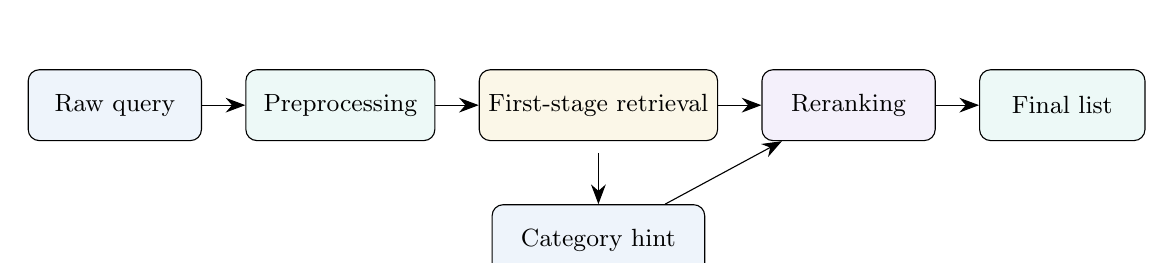
\begin{tikzpicture}[node distance=0.8cm and 0.55cm, every node/.style={font=\small}]
\node[draw,rounded corners,fill=SoftBlue,minimum width=2.2cm,minimum height=0.9cm] (a) {Raw query};
\node[draw,rounded corners,fill=SoftTeal,right=of a,minimum width=2.4cm,minimum height=0.9cm] (b) {Preprocessing};
\node[draw,rounded corners,fill=SoftGold,right=of b,minimum width=2.6cm,minimum height=0.9cm] (c) {First-stage retrieval};
\node[draw,rounded corners,fill=SoftPurple,right=of c,minimum width=2.2cm,minimum height=0.9cm] (d) {Reranking};
\node[draw,rounded corners,fill=SoftBlue,below=of c,minimum width=2.7cm,minimum height=0.9cm] (e) {Category hint};
\node[draw,rounded corners,fill=SoftTeal,right=of d,minimum width=2.1cm,minimum height=0.9cm] (f) {Final list};
\draw[-{Stealth[length=2.5mm]}] (a) -- (b);
\draw[-{Stealth[length=2.5mm]}] (b) -- (c);
\draw[-{Stealth[length=2.5mm]}] (c) -- (d);
\draw[-{Stealth[length=2.5mm]}] (d) -- (f);
\draw[-{Stealth[length=2.5mm]}] (e) -- (d);
\draw[-{Stealth[length=2.5mm]}] ([yshift=-1.5mm]c.south) -- (e.north);
\end{tikzpicture}
\end{center}

\begin{warningbox}
Notice how each stage adds something different: preprocessing adds consistency, retrieval adds coverage, reranking adds precision, and category adjustment adds a weak topical prior.
\end{warningbox}

\begin{selfcheckbox}
\textbf{1.} Which stage first narrows the huge corpus to a manageable shortlist?\\
\textbf{2.} Which stage is most likely to move one candidate above another inside that shortlist?\\
\textbf{3.} Why is category adjustment described as weak rather than decisive?
\end{selfcheckbox}

\begin{answerbox}
\textbf{1.} First-stage retrieval.\\
\textbf{2.} Reranking.\\
\textbf{3.} Because category is only a supporting signal; exact relevance should still dominate the decision.
\end{answerbox}

\begin{rememberbox}
A useful mental image is: preprocess for consistency, retrieve for coverage, rerank for sharper judgment, and then evaluate the final ordering.
\end{rememberbox}


\chapter[Full Pipeline Mental Model]{Full pipeline mental model}

\begin{purposebox}
This final chapter integrates the full learning path. Its goal is not to introduce new terminology, but to connect every major component into one coherent system-level understanding.
\end{purposebox}

\section*{End-to-end summary}
A retrieval pipeline begins with text representation. Raw documents and queries are normalized and turned into forms that models can use. Sparse lexical models such as TF--IDF and BM25 measure weighted token overlap. Dense semantic models such as bi-encoders map texts into an embedding space where paraphrases can still be close. Because first-stage retrieval must remain scalable, it often serves as a candidate generator. A second-stage reranker, especially a cross-encoder, can then inspect the best candidates more carefully. A classifier may provide a soft topical hint. Evaluation separates training, validation, holdout checking, and final unlabeled submission. Engineering makes the whole process practical through caching, chunking, and efficient top-$k$ selection.

\section*{What each stage adds}
\begin{center}
\begin{tabularx}{\textwidth}{>{\bfseries}lY}
\toprule
Stage & Main contribution \\
\midrule
Preprocessing & Consistent text representation \\
Sparse lexical retrieval & Strong exact-token matching and transparency \\
Dense bi-encoder retrieval & Better semantic coverage and paraphrase recovery \\
Candidate set & Makes later expensive judgment possible \\
Cross-encoder reranking & Better local precision among plausible candidates \\
Category classifier & Weak topical prior or soft bonus \\
Validation and holdout protocol & Honest selection and credible reporting \\
Engineering & Feasible runtime and reproducible experimentation \\
\bottomrule
\end{tabularx}
\end{center}

\section*{When each method helps most}
Use lexical methods when exact terms, codes, flags, and commands matter. Use dense retrieval when wording varies and paraphrase mismatch is common. Use reranking when the first stage is good at finding plausible candidates but not perfect at ordering them. Use category information when topical boundaries exist and can help guide near-ties.

\section*{Final integrated diagram}
\begin{center}
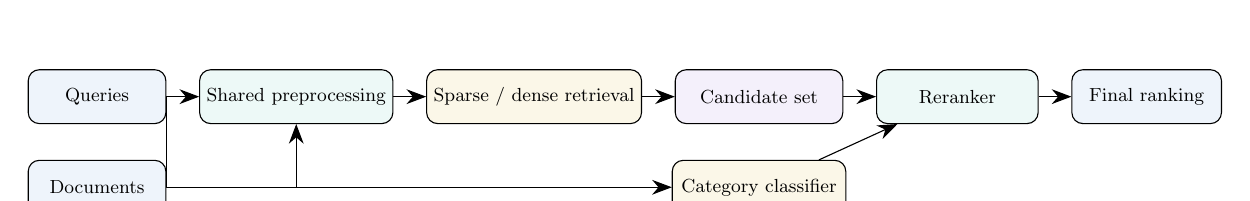
\begin{tikzpicture}[scale=0.76,transform shape,node distance=0.6cm and 0.55cm, every node/.style={font=\small}]
\node[draw,rounded corners,fill=SoftBlue,minimum width=2.3cm,minimum height=0.9cm] (q) {Queries};
\node[draw,rounded corners,fill=SoftBlue,below=of q,minimum width=2.3cm,minimum height=0.9cm] (d) {Documents};
\node[draw,rounded corners,fill=SoftTeal,right=of q,minimum width=2.8cm,minimum height=0.9cm] (p1) {Shared preprocessing};
\node[draw,rounded corners,fill=SoftGold,right=of p1,minimum width=3.0cm,minimum height=0.9cm] (r1) {Sparse / dense retrieval};
\node[draw,rounded corners,fill=SoftPurple,right=of r1,minimum width=2.8cm,minimum height=0.9cm] (cset) {Candidate set};
\node[draw,rounded corners,fill=SoftTeal,right=of cset,minimum width=2.7cm,minimum height=0.9cm] (re) {Reranker};
\node[draw,rounded corners,fill=SoftGold,below=of cset,minimum width=2.9cm,minimum height=0.9cm] (cls) {Category classifier};
\node[draw,rounded corners,fill=SoftBlue,right=of re,minimum width=2.5cm,minimum height=0.9cm] (fin) {Final ranking};
\draw[-{Stealth[length=2.5mm]}] (q) -- (p1);
\draw[-{Stealth[length=2.5mm]}] (d.east) -| (p1.south);
\draw[-{Stealth[length=2.5mm]}] (p1) -- (r1);
\draw[-{Stealth[length=2.5mm]}] (r1) -- (cset);
\draw[-{Stealth[length=2.5mm]}] (cset) -- (re);
\draw[-{Stealth[length=2.5mm]}] (re) -- (fin);
\draw[-{Stealth[length=2.5mm]}] (q.east) |- (cls.west);
\draw[-{Stealth[length=2.5mm]}] (cls) -- (re);
\end{tikzpicture}
\end{center}

\section*{Final advice for studying}
On your next pass through the notebook, do not ask ``what does this line of code do?'' first. Ask ``which part of the pipeline is this line serving?'' That shift in perspective is what turns the notebook from a wall of implementation details into a system you can reason about.

\begin{selfcheckbox}
\textbf{1.} In one sentence, what is the main job of first-stage retrieval?\\
\textbf{2.} In one sentence, what is the main job of reranking?\\
\textbf{3.} Why is evaluation protocol part of the pipeline, not only an external report?
\end{selfcheckbox}

\begin{answerbox}
\textbf{1.} First-stage retrieval must search the large corpus efficiently and keep a candidate set with good coverage.\\
\textbf{2.} Reranking must reorder those candidates more precisely using a stronger but more expensive relevance signal.\\
\textbf{3.} Because the meaning of every reported result depends on where the decisions were made and how tuning was controlled.
\end{answerbox}

\begin{rememberbox}
The full pipeline is a division of labor: represent text well, retrieve broadly, rerank carefully, use category only as support, evaluate honestly, and engineer the system so it can actually run.
\end{rememberbox}



\chapter*{Part I glossary}
\addcontentsline{toc}{chapter}{Part I glossary}
\begin{longtable}{p{0.24\textwidth}p{0.70\textwidth}}
\toprule
\textbf{Term} & \textbf{Meaning in plain language} \\ \midrule
Data & Recorded examples or observations that a system can use. \\ \midrule
Feature & A measurable description of an example. \\ \midrule
Label & The outcome or target we want to predict. \\ \midrule
Model & A mathematical rule that maps input to output. \\ \midrule
Training & The process of fitting a model from past examples. \\ \midrule
Prediction & Using a fitted model on a new example. \\ \midrule
Token & A unit of text used by the system, often a word or word-piece. \\ \midrule
Normalization & Making text more consistent before later steps. \\ \midrule
Preprocessing & The broader text-preparation stage. \\ \midrule
Vector & An ordered list of numbers. \\ \midrule
Matrix & A table of numbers, often many vectors stacked together. \\ \midrule
Sparse & Mostly zero. \\ \midrule
Dense & Many non-zero entries carrying signal together. \\
\bottomrule
\end{longtable}


\chapter*{Part II glossary}
\addcontentsline{toc}{chapter}{Part II glossary}
\begin{longtable}{p{0.24\textwidth}p{0.70\textwidth}}
\toprule
\textbf{Term} & \textbf{Meaning in plain language} \\ \midrule
Corpus & The full searchable document collection. \\ \midrule
Query & The search request or problem statement. \\ \midrule
Document & One searchable item in the corpus. \\ \midrule
Relevance & Whether a document truly helps answer the query. \\ \midrule
Ranking & The ordered list returned by the system. \\ \midrule
Top-k & The first k highest-ranked results. \\ \midrule
Lexical matching & Matching based mainly on token overlap. \\ \midrule
Semantic matching & Matching based on closeness in meaning. \\ \midrule
Vocabulary mismatch & A relevant query-document pair using different words. \\
\bottomrule
\end{longtable}


\chapter*{Part III glossary}
\addcontentsline{toc}{chapter}{Part III glossary}
\begin{longtable}{p{0.24\textwidth}p{0.70\textwidth}}
\toprule
\textbf{Term} & \textbf{Meaning in plain language} \\ \midrule
Bag of words & A text view that keeps token counts and mostly ignores order. \\ \midrule
TF & Term frequency inside one document. \\ \midrule
DF & Number of documents containing a term. \\ \midrule
IDF & Inverse document frequency; a weight that grows for rarer terms. \\ \midrule
TF--IDF & A sparse weighting scheme combining within-document frequency and corpus rarity. \\ \midrule
BM25 & A lexical ranking function with term-frequency saturation and length normalization. \\ \midrule
BM25+ & A refinement of BM25 with a positive offset to reduce over-penalization. \\
\bottomrule
\end{longtable}


\chapter*{Part IV glossary}
\addcontentsline{toc}{chapter}{Part IV glossary}
\begin{longtable}{p{0.24\textwidth}p{0.70\textwidth}}
\toprule
\textbf{Term} & \textbf{Meaning in plain language} \\ \midrule
Embedding & A dense learned vector representation of text. \\ \midrule
Bi-encoder & A model that encodes query and document separately. \\ \midrule
Dense retrieval & Retrieval based on learned dense vectors and similarity search. \\ \midrule
Similarity search & Finding items whose vectors are close to a query vector. \\ \midrule
Recall-oriented\\candidate generator & A first-stage retriever that aims to keep many relevant items in the shortlist. \\
\bottomrule
\end{longtable}


\chapter*{Part V glossary}
\addcontentsline{toc}{chapter}{Part V glossary}
\begin{longtable}{p{0.24\textwidth}p{0.70\textwidth}}
\toprule
\textbf{Term} & \textbf{Meaning in plain language} \\ \midrule
Reranker & A second-stage model that reorders a candidate set. \\ \midrule
Candidate set & The shortlist of documents passed from retrieval to later stages. \\ \midrule
Cross-encoder & A model that reads the query-document pair jointly and outputs one score. \\ \midrule
Positive pair & A query paired with a relevant document. \\ \midrule
Negative pair & A query paired with a non-relevant document. \\ \midrule
Hard negative & A plausible but still non-relevant document, often mined from retrieval mistakes. \\
\bottomrule
\end{longtable}


\chapter*{Part VI glossary}
\addcontentsline{toc}{chapter}{Part VI glossary}
\begin{longtable}{p{0.24\textwidth}p{0.70\textwidth}}
\toprule
\textbf{Term} & \textbf{Meaning in plain language} \\ \midrule
Classification & Predicting a category label for one input example. \\ \midrule
Category prior & A weak expectation about which topical region is more likely. \\ \midrule
Soft bonus & A small score increase rather than a hard removal. \\ \midrule
Hard filtering & Removing candidates that fail a category condition. \\ \midrule
Linear classifier & A model using weighted sums of input features to score classes. \\ \midrule
LinearSVC & A classical linear support-vector classifier often used with TF--IDF features. \\
\bottomrule
\end{longtable}


\chapter*{Part VII glossary}
\addcontentsline{toc}{chapter}{Part VII glossary}
\begin{longtable}{p{0.24\textwidth}p{0.70\textwidth}}
\toprule
\textbf{Term} & \textbf{Meaning in plain language} \\ \midrule
Precision & Fraction of returned results that are relevant. \\ \midrule
Recall & Fraction of all relevant results that were recovered. \\ \midrule
F1 & A balance of precision and recall. \\ \midrule
Reciprocal rank & Inverse of the rank of the first relevant result. \\ \midrule
MRR & Mean reciprocal rank across many queries. \\ \midrule
Validation split & Held-out labeled data used for model and hyperparameter selection. \\ \midrule
Holdout split & A later protected labeled check after selection. \\ \midrule
Leakage & Unwanted flow of evaluation information into training or tuning. \\ \midrule
Hyperparameter & A system setting chosen by the experimenter rather than directly learned by fitting. \\
\bottomrule
\end{longtable}


\chapter*{Part VIII glossary}
\addcontentsline{toc}{chapter}{Part VIII glossary}
\begin{longtable}{p{0.24\textwidth}p{0.70\textwidth}}
\toprule
\textbf{Term} & \textbf{Meaning in plain language} \\ \midrule
Caching & Saving reusable artifacts instead of recomputing them. \\ \midrule
Chunking & Breaking a large computation into smaller pieces. \\ \midrule
Partial sorting & Finding only the top region instead of fully sorting everything. \\ \midrule
Pipeline & The sequence of stages that turn raw inputs into final outputs. \\
\bottomrule
\end{longtable}


\appendix
\chapter{Final cheat sheet}
\begin{purposebox}
This cheat sheet is not a substitute for the full guide. It is a memory aid for your second or third pass.
\end{purposebox}

\section*{Core distinctions}
\begin{itemize}
\item Retrieval ranks documents for a query; classification predicts a category for one input.
\item Sparse representations emphasize lexical overlap; dense representations emphasize learned semantic closeness.
\item Bi-encoders scale to large corpora; cross-encoders usually rerank shortlists.
\item Validation chooses settings; holdout checks the chosen system; unlabeled test is for final output, not offline tuning.
\end{itemize}

\section*{Formula reminders}
\begin{align*}
\mathrm{tfidf}(t,d) &= \mathrm{tf}(t,d)\cdot \mathrm{idf}(t) \\
\mathrm{idf}(t) &= \log\!\left(\frac{N}{df(t)}\right) \\
\cos(\theta) &= \frac{\vect{q}\cdot\vect{d}}{\|\vect{q}\|\,\|\vect{d}\|} \\
\mathrm{Precision@K} &= \frac{|R_q\cap \hat{R}_{q,K}|}{K} \\
\mathrm{Recall@K} &= \frac{|R_q\cap \hat{R}_{q,K}|}{|R_q|} \\
\mathrm{RR}(q) &= \frac{1}{r_q}
\end{align*}

\section*{Pipeline memory line}
\begin{rememberbox}
Represent text well, retrieve broadly, rerank carefully, use classification softly, evaluate honestly, and engineer for runtime.
\end{rememberbox}


\chapter*{Master glossary}
\addcontentsline{toc}{chapter}{Master glossary}
\begin{longtable}{p{0.24\textwidth}p{0.70\textwidth}}
\toprule
\textbf{Term} & \textbf{Meaning in plain language} \\ \midrule
Bag of words & Count-based text view that mostly ignores order. \\ \midrule
Batch size & How many examples are processed together in one step. \\ \midrule
Bi-encoder & Separate query/document encoder architecture for scalable semantic retrieval. \\ \midrule
BM25 & Lexical ranking model with saturation and length normalization. \\ \midrule
BM25+ & BM25 with a positive offset to reduce over-penalization. \\ \midrule
Candidate set & Shortlist passed to later stages. \\ \midrule
Category bonus & Small score increase when category agreement occurs. \\ \midrule
Classification & Predicting a discrete label for one example. \\ \midrule
Corpus & Complete searchable document collection. \\ \midrule
Cosine similarity & Alignment-based similarity between vectors. \\ \midrule
Cross-encoder & Pairwise joint-reading reranker. \\ \midrule
Dense vector & Representation with many non-zero values. \\ \midrule
Embedding & Dense learned vector for text. \\ \midrule
Feature & Input description used by a system. \\ \midrule
Hard negative & Plausible but wrong document used in training. \\ \midrule
Holdout & Protected later evaluation split. \\ \midrule
Hyperparameter & Experimenter-chosen setting such as top-k or bonus strength. \\ \midrule
IDF & Inverse document frequency. \\ \midrule
\bottomrule
\end{longtable}

\clearpage
\begin{center}
\textbf{Master glossary (continued)}
\end{center}
\begin{longtable}{p{0.24\textwidth}p{0.70\textwidth}}
\toprule
\textbf{Term} & \textbf{Meaning in plain language} \\ \midrule
Leakage & Improper use of evaluation information during training or tuning. \\ \midrule
MRR & Mean reciprocal rank. \\ \midrule
Normalization & Making text more consistent. \\ \midrule
Precision & How clean returned results are. \\ \midrule
Query & The search request. \\ \midrule
Recall & How much relevant material was recovered. \\ \midrule
Retrieval & Ranking documents for a query. \\ \midrule
Reranker & Second-stage model that reorders a candidate set. \\ \midrule
Sparse vector & Vector with mostly zero entries. \\ \midrule
TF & Term frequency. \\ \midrule
TF--IDF & Sparse lexical weighting scheme. \\ \midrule
Token & Text unit used by the system. \\ \midrule
top-k & Number of candidates retained after a stage. \\ \midrule
top-m & Number of candidates passed to an expensive reranker. \\ \midrule
Validation & Split used to choose settings honestly. \\ \midrule
Vocabulary mismatch & Relevant texts using different words. \\ \midrule
Vector & Ordered list of numbers. \\
\bottomrule
\end{longtable}

\end{document}
